\documentclass[russian, utf8, emptystyle]{eskdtext}
\usepackage{amsmath, amsthm, amssymb, amsfonts, footnote, titlesec, epstopdf, tabularx}
\newcolumntype{L}[1]{>{\raggedright\let\newline\\\arraybackslash\hspace{0pt}}m{#1}}
\newcolumntype{C}[1]{>{\centering\let\newline\\\arraybackslash\hspace{0pt}}m{#1}}   \newcolumntype{R}[1]{>{\raggedleft\let\newline\\\arraybackslash\hspace{0pt}}m{#1}}

\newcommand{\sectionbreak}{\clearpage}

\newcommand*\justify{%
	\fontdimen2\font=0.4em% interword space
	\fontdimen3\font=0.2em% interword stretch
	\fontdimen4\font=0.1em% interword shrink
	\fontdimen7\font=0.1em% extra space
	\hyphenchar\font=`\-% allowing hyphenation
}

%\let\oldsection\section

%\renewcommand{\section}{\pagebreak \oldsection}

\setlength{\footskip}{20pt}
\begin{document}
\thispagestyle{empty}

\begin{center}
	\ \vspace{-2cm}
	
	
\includegraphics[width=0.5\textwidth]{msu.jpg}\\
	{\scshape Московский государственный университет \\ имени М.В.~Ломоносова}\\
	Факультет вычислительной математики и кибернетики\\
	Кафедра  автоматизации систем вычислительных комплексов
	
	\vspace{4cm}
	
	\textbf{{\Large Треско Константин Игоревич}}
	
	\vspace{1cm}
	
	{\Huge\bfseries
	Исследование и разработка средств многотемной классификации веб-страниц\\}
\end{center}

\vspace{1cm}

\center{{\normalsize ВЫПУСКНАЯ КВАЛИФИКАЦИОННАЯ РАБОТА}}

\vspace{2cm}

\vfill

\begin{flushright}
	\normalsize
	\textbf{Научные руководители:}\\
	к.ф.-м.н. М.И. Петровский\\
	Д.В. Царев
\end{flushright}

\vfill

\begin{center}
	Москва, 2015
\end{center}

\enlargethispage{4\baselineskip}


	
\newpage
\abstract{
	Целью данной работы является исследование и разработка экспериментального прототипа системы сбора и многотемной классификации веб-страниц, с которыми работали пользователи, находящиеся внутри одной сети. Отличие многотемной классификации заключается в том, что классы могут пересекаться или даже быть вложенными. 
	
	Разрабатываемая система сбора должна удовлетворять требованиям масштабируемости (линейного роста расхода ресурсов при увеличении числа подключений) и защищенности (пользователь не должен иметь возможности фальсифицировать собранные данные). Модуль классификации данных должен обеспечивать многотемную классификацию на основе машинного обучения с возможностью добавления и удаления тематик.
	
	В ходе работы был проведен обзор существующих средств многотемной классификации и средств реализации системы сбора. Также был реализован экспериментальный прототип системы сбора и многотемной классификации, удовлетворяющий поставленным выше требованиям, проведено тестирование, показавшее масштабируемость и защищенность разработанного средства.	
}
\section {Введение}

\subsection {Задача классификации}
Настоящая работа посвящена исследованию и разработке программных средств сбора и многотемной классификации текстовых данных веб-страниц. Задача классификации многотемных документов (multi-label classification), заключается в определении принадлежности документа к одному или нескольким классам (из предопределённого набора классов) на основании анализа совокупности признаков, характеризующих данный документ. В отличие от традиционной задачи классификации, классы могут пересекаться или быть вложенными, то есть документ может принадлежать нескольким классам. Классы, к которым принадлежит документ называются релевантными.
\begin{figure}[h]
	\begin{center}
		\includegraphics[width=14cm]{pic/ML_Classification.png}
		\caption{Многотемная и многоклассовая классификация}
		\label{fig:low_sigma}
	\end{center}
\end{figure}
\subsection {Области применения классификации веб-данных}
На сегодняшний день существует ряд задач, для решения которых требуются системы сбора и классификации контента, частным случаем которого является веб-контент:
\begin{itemize}
	\item {\bf Анализ работы сотрудников организации.}
	Определение тематик документов, с которыми работает пользователь. На основе полученной информации применение политик безопасности.
	\item {\bf Фильтрации контента, для обнаружения информации, относящейся к определенному делу (eDiscovery\cite{eDiscovery}).}
	Документы и электронная почта могут фильтроваться в зависимости от присвоенных им классов, чтобы гарантировать, что только материалы с запрошенной бизнес-информацией в рамках расследуемого дела были найдены и сохранены.
	\item {\bf Определения конфиденциальности документа, для предотвращения утечек информации}
	По различным экспертным оценкам в настоящее время наибольшие риски для информационной безопасности представляют не внешние, а внутренние угрозы \cite{InfoWatch}.
	Поэтому существует необходимость в средствах определения конфиденциальности документа.
	
\end{itemize}

Далее будут рассмотрены классы индустриальных систем, функционал которых включает в себя классификацию текстовых данных (в том числе веб-данных), с которыми работают пользователи.
\begin{itemize}
	\item {\bf 	Системы управления корпоративным контентом (англ. Enterprise Content Management, ECM) } - программные решения для управления информационными ресурсами предприятия предоставляют программные средства сбора, анализа, управления, накопления, хранения и доставки документов в масштабах организации. В настоящее время большинство ECM систем включают в себя системы обнаружения данным, связанных с определенным судебным делом (англ. eDiscovery). Средства eDiscovery обеспечивают процесс, с помощью которого организации находят, получают, сохраняют и анализируют документы, связанные с делом.
	\item {\bf Системы предотвращения утечки данных (англ. Data Loss Prevention, DLP)} -
	программные решения для предотвращения утечек конфиденциальной информации и минимизации других рисков, связанных с внутренними угрозами.
\end{itemize}
\subsection{Основные методы сбора и классификации данных в корпоративных системах}
Поиск и анализ информации в ECM системах происходит следующим образом:
\begin{itemize}
	\item {\bf Сбор данных.} Системы сбора содержат компоненту, установленную на пользовательском компьютере и отвечающую за мониторинг деятельности пользователя. В терминологии IBM данные компоненты называются Искателями \cite{searcher}.
	\item {\bf Применение методов анализа документов.} В терминологии IBM данный этап называется аналитическим конвейером \cite{analitic}.
	\item {\bf Индексация данных.} Компоненты индексации добавляют в индекс информацию о новых и измененных документах
	\cite{idx1,idx2,idx3}.
\end{itemize}

Существуют три основных подхода к классификации данных в ECM системах
\begin{itemize}
	\item {\bf Классификация на основе обучающей выборки} (IBM Content Classification \cite{ContentClassification}, Symantec eDiscovery \cite{Symantec}).
	\item {\bf Классификация на основе заданных правил}. Принадлежность документа к тому или иному классу определяется на основе эвристических правил (сигнатур). Правила могут формироваться на основе контекста – имя отправителя, директория создания и т.п., а также на основе контента – шаблоны текста, ключевые слова и т.п. 
	\item {\bf Определение категорий в неизвестных документах}.
	В задаче кластеризации нет предопределенного набора классов. Исходное множество документов разбивается на подмножество таким образом, чтобы документы в различных подмножествах существенно отличались.
\end{itemize}


В DLP системах выделяют следующие технологии классификации данных:
\begin{itemize}
	\item {\bf Цифровые отпечатки (англ. digital fingerprint)} - технология предназначена для защиты больших по объему документов, содержание которых не изменяется или меняется незначительно. Детектор цифровых отпечатков позволяет автоматически обнаруживать в анализируемом тексте цитаты из документов-образцов, содержащих конфиденциальную информацию.
	\item {\bf Анализ шаблонов} - технология предназначена для детектирования алфавитно-цифровых объектов по шаблону данных (маске) и позволяет наиболее эффективно выявлять факты пересылки персональных данных или финансовой информации. Кроме того, данная технология может использоваться как вспомогательный метод для обнаружения фактов несанкционированной пересылки внутренних документов, содержащих формализованные данные, образованные по определенному шаблону (например, договоров или счетов в случае детектирования банковских реквизитов, кодов классификаторов и т.д.).
	\item {\bf Машинное обучение} (InfoWatch \cite{bkf}, Symantec VML \cite{MachLearn}). Примерная схема работы классификатора такова: на вход подается обучающий набор документов, состоящий как из конфиденциальных так и не конфиденциальных документов. По этим наборам производится обучение и строится статистическая модель. Далее полученная модель используется для классификации неизвестным документов. При обнаружении конфиденциального документа производятся действия, предписанные политиками безопасности.
\end{itemize}
\begin{table} 
	\caption{Подходы к классификации}
	\label{tab:far}
	\begin{center}
		\begin{tabular}{|L{5cm}|L{5cm}|L{5cm}|}
			\hline
			& Достоинства & Недостатки \\
			\hline     
			Цифровые отпечатки - обнаружение в тексте цитат из документов-образцов
			& Высокая точность детектирования статичных документов
			& Чувствительность к текстовым изменениям\\
			\hline
			Анализ шаблонов - анализ текстов на основе словарей и регулярных выражений
			& Эффективность в детектировании формализованных данных
			& Не применим для детектирования неформализованных данных\\
			\hline
			Машинное обучение – построение на основе обучающего набора статистической модели
			& Работают напрямую с содержимым документов
			Обучаемость
			Возможность обобщения
			& Требуется формирование обучающего набора
			Возможность ложноотрицательных и ложноположительные срабатываний
			Возможность обобщения \\
			\hline
		\end{tabular}
	\end{center}
\end{table}
Основное преимущество машинного обучения заключается в том, что в отличие от других описанных технологий, оно предназначено для работы не со статическими, а с постоянно меняющимися документами.\\
\subsection{Специфика задачи классификации текстовых веб-данных}

Веб – страницы имеют следующие особенности:
\begin{itemize}
	\item Содержимое веб-страниц постоянно меняется.
	\item Содержимое имеет многотемную природу, то есть каждая  из страниц может одновременно принадлежать к нескольким тематикам.
\end{itemize}
	\begin{figure}[h]
		\begin{center}
			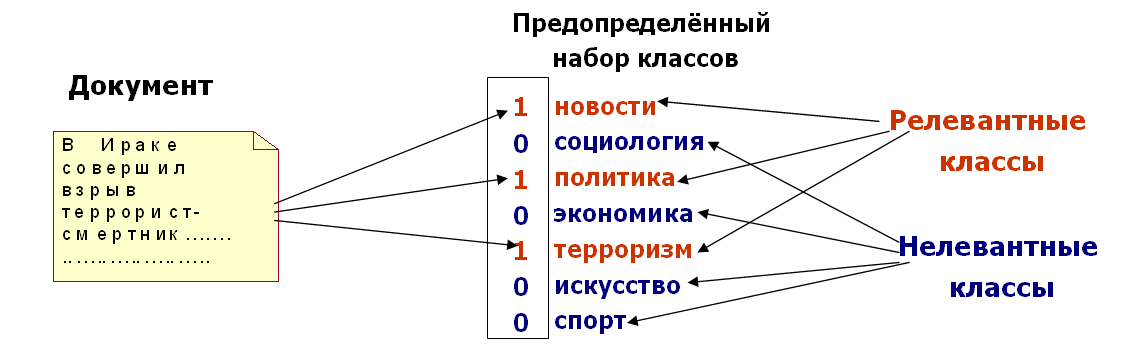
\includegraphics[width=14cm]{pic/Nature.png}
			\caption{Многотемная природа документа}
			\label{fig:low_sigma}
		\end{center}
	\end{figure}
\subsection{Выводы}
На сегодняшний день существует ряд прикладных задач, требующих классификации текстовых данных. Обзор индустриальных систем показал, что наиболее актуальными технологиями классификации текстовых данных являются:
\begin{itemize}
	\item Метод шаблонов.
	\item Метод цифровых отпечатков.
	\item Метод машинного обучения.
\end{itemize}

Первые две технологии применимы только к статическим данным, в то время как метод машинного обучения позволяет позволять адаптироваться к тому, что содержимое и состав анализируемых данных постоянно меняется.\\
Для задачи классификации текстовых веб–данных из рассмотренных технологий подходит только машинное обучение с возможностью дообучения, так как веб – данные и набор классов постоянно меняются. \\
Рассмотренные системы решают задачу многоклассовой классификации, так как документ может принадлежать только к одному из предопределенного набора классу. Так как большая часть веб – данных имеет многотемную природу, то существует актуальность разработки системы сбора и многотемной классификации текстовых веб - данных пользователей. С учетом большого объема анализируемой информации к модулю классификации предъявляется требование масштабируемости. \\

Так как в рассмотренных системах присутствуют компоненты сбора информации, расположенные на пользовательских машинах, то при разработке системы сбора нужно учитывать то, что деятельность компонент никак не должна сказываться на работе пользователя. Также в рассмотренных системах пользователь не имеет доступа к собираемой информации, поэтому система сбора должна удовлетворять требованию защищенности.
\section{Постановка задачи}
Разработать архитектуру и реализовать прототип системы сбора и многотемной классификации текстовых веб-данных пользователя в соответствии  с требованиями:
\begin{itemize}
	\item Модуль сбора должен обеспечивать:
	\begin{itemize}
		\item Масштабируемость (линейный рост расхода ресурсов при росте числа подключений).
		\item Защищенность (пользователь не должен иметь возможности фальсифицировать данные).
		\item Функционирование под ОС Windows и браузером IE. 
	\end{itemize}
	\item Модуль классификации должен обеспечивать:
		\begin{itemize}
			\item Многотемную классификацию на основе машинного обучения с возможностью дообучения.
			\item Возможность добавления и удаления тематик.
		\end{itemize}
\end{itemize}
\section{Обзор}
Для реализации прототипа системы многотемной классификации веб-страниц, с которыми работал пользователь необходимо осуществить:
\begin{itemize}
	\item {\bf Сбор} просмотренных пользователем веб-страниц.
	\item {\bf Модуль классификации}, который будет определять принадлежность документа предопределенным классам.
\end{itemize}

Компонента модуля сбора будет установленна на каждой из пользовательских машин и будет состоять из:
\begin{itemize}
	\item Расширения для браузера, сохраняющего html код просматриваемой пользователем веб – страницы в локальную базу данных, расположенную на пользовательском компьютере.
	\item Модуля сбора данных.
\end{itemize}
\subsection{Расширение для браузера}
Для решения задачи необходимо расширение для браузера, имеющее возможность сохранить html код просматриваемой пользователем веб – страницы в локальную базу данных, без подтверждения пользователем.
\begin{itemize}
	\item {\bf BHO} (Browser Helper Object) - DLL-модуль, разработанный как плагин для Internet Explorer для обеспечения дополнительной функциональности. В BHO API существует возможность получения доступа к DOM (Document Object Model\cite{DOM}) текущей страницы. Также существует возможность обработки событий и управления навигацией. Для задачи перехвата контента данное решение подходит. Минусом является то, что данное решение подходит только для браузера IE. Но BHO имеет возможность записи и чтения данных из файловой системы пользователя, без его участия.
	\item {\bf Kynext} позволяет перехватывать содержимое веб – страницы. Поддерживает IE, Firefox, Safari, and Chrome, но для написания необходимо использовать проприетарный язык Kynetx Rules Language. Еще одним минусом является то, что работа написанного расширение зависит от работоспособности самого расширения Kynext.
	\item {\bf WebMynd} поддерживает  IE, Firefox, Safari, and Chrome. Пока доступна бета версия, и не известно, будет ли дальнейшая поддержка продукта. Поддерживает JavaScript API. Не является бесплатным программным обеспечением.
	\item {\bf Crossrider} позволяет быстро создавать кросс-браузерные расширения. Использует один API и поддерживает JavaScript и jQuery, так что разработчик с базовыми знаниями JavaScript может писать и поддерживать свой код. Имеется возможность писать под IE, Firefox, Safari, and Chrome. Бесплатен в использовании. Существует документация и демо – видео для некоторых задач. Доступ к файловой системе пользователя только с его разрешения. 
\end{itemize}
\begin{table} 
	\caption{Средства расширения для браузера}
	\label{tab:far}
	\begin{center}
		\begin{tabular}{|L{5cm}|L{2cm}|L{2cm}|L{2cm}|L{2cm}|}
			\hline
			& BHO & Crossrider & Kynext & WebMynd \\
			\hline     
			Кроссплатформеность  & -(только IE) & + & + & + \\
			\hline
			Бесплатность & + & + & + & -\\
			\hline
			Поддерживаемые языки & C++,C\# & JavaScript & Kynext Rules Language & JavaScript  \\
			\hline
			Возможность записи в локальную ФС & + & - & - &- \\
			\hline
		\end{tabular}
	\end{center}
\end{table}
\subsection{Методы многотемной классификации}
Можно выделить три основных подхода к многотемной классификации: \cite{dis}
\begin{itemize}
	\item «Оптимизационный» подход \cite{AdaBoost,ADT,mlKNN}.
	\item Подход на основе декомпозиции в набор независимых бинарных проблем. 
	\item Подход на основе ранжирования \cite{rank1,rank2}.
\end{itemize}
	\subsubsection{Методы, основанные на "оптимизационном"  подходе}
К числу алгоритмов, использующих данный подход, относятся алгоритмы, решающие оптимизационную задачу. Рассмотрим некоторые из данных алгоритмов:
\begin{itemize}
	\item Основанные на AdaBoost алгоритме (AdaBoost.MH \cite{AdaBoost},ADTBoost.MH \cite{ADT}) - минимизируется функция Hamming Loss), где $$HammingLoss=\frac{1}{k}\sum_{i=1}^{k-1}\frac{1}{|Y|}|(f_Z(x_i))\nabla(y_i)|$$
	где $a\nabla(b)=(a\cup b) \setminus (a \cap b), a \subseteq Y, b \subseteq Y$, k - размер тестового набора. Другими словами, критерий   оценивает, сколько раз пара «пример-метка» классифицируется не правильно. 
	\item Multi-Label-kNN - \cite{kNN} максимизируются апостериорные вероятности принадлежности классам
\end{itemize}.
{\bf Методы, основанные на алгоритме AdaBoost.} К числу данных методов можно отнести AdaBoost.MH \cite{AdaBoost} и ADTBoost.MH \cite{ADT}.
AdaBoost вызывает слабые классификаторы в цикле  $t = 1,\ldots,T.$ После каждого вызова обновляется распределение весов $D_{t}$, которые отвечают важности каждого из объектов обучающего множества для классификации. На каждой итерации веса каждого неверно классифицированного объекта возрастают, таким образом новый комитет классификаторов «фокусирует своё внимание» на этих объектах.

Алгоритм работы AdaBoost \cite{wikiAdaBoost}:

Дано: $(x_{1},y_{1}),\ldots,(x_{m},y_{m}) где x_{i} \in X,\, y_{i} \in Y = \{-1, +1\}$

Изначально присваиваем всем классам одинаковый вес $D_{t}(i) = \frac{1}{m}, i=1,\ldots,m.$
$for~t = 1, \ldots, T$
\begin{itemize}
	\item Находим классификатор, минимизирующий взвшенную ошибку классификации $ h_{t} = \arg \min_{h_{j} \in \mathcal{H}} \epsilon_{j}$, где  $\epsilon_{j} = \sum_{i=1}^{m} D_{t}(i)[y_i \ne h_{j}(x_{i})]$.
	\item Если величина $\epsilon_{t} \geqslant 0.5$, то останавливаемся.
	\item Выбираем $\alpha_{t} \in \mathbf{R}$, обычно $\alpha_{t}=\frac{1}{2}\textrm{ln}\frac{1-\epsilon_{t}}{\epsilon_{t}}$, где $\epsilon_{t}$ взвешенная ошибка классификатора $h_{t}$.
	\item $D_{t+1}(i) = \frac{ D_{t}(i) \, e^{- \alpha_{t} y_{i} h_{t}(x_{i})} }{ Z_{t} }$, где где $Z_{t}$ является нормализующим параметром (выбранным так, чтобы $D_{t+1}$ являлось распределением вероятностей, то есть $\sum_{i=1}^{m} D_{t+1}(i) = 1)$.
\end{itemize}

Итоговый классификатор имеет вид: $H(x) = \textrm{sign}\left( \sum_{t=1}^{T} \alpha_{t}h_{t}(x)\right)$

Таким образом, на каждом шаге выбирается оптимальный классификатор, и веса тех объектов $x_i$, которые он предсказал правильно, уменьшаются, а тех, которые он предсказал неверно - увеличиваются, чтобы на следующем шаге был выбран классификатор, который лучше распознает объекты, неверно распознанные предыдущим.

С точки зрения сформулированных требований метод AdaBoost имеет следующие недостатки:
\begin{itemize}
	\item Алгоритм не имеет возможности пошагового дообучения, поскольку принцип работы метода рассчитан на то, что обучающий набор задан заранее целиком.
	\item Для достижения качества классификации, удовлетворяющего потребностям актуальных прикладных задач, этот метод требует большое число шагов на этапе обучения, а следовательно, обучение выполняется достаточно долго.
\end{itemize}

В случае многотемного AdaBoost заключительная гипотеза для ранжирования классов получается как взвешенное голосование слабых гипотез(гипотез, полученных при решении задачи многоклассовой классификации), причём вес слабой гипотезы вычисляются с учётом качества классификации этой гипотезой примеров из обучающего набора. Заключительная гипотеза multi-label классификации получается на основе гипотезы ранжирования путём отсечения по нулевому порогу релевантности.

{\bf Multi-Label-kNN.} Данный метод представляет собой подход многотемного обучения, основанный на методе k ближайших соседей.
Основным принципом метода ближайших соседей является то, что объект присваивается тому классу, который является наиболее распространённым среди соседей данного элемента.
В многотемном варианте kNN расстояние выражается через косинус угла между векторами признаков элементов: $\rho = 1 - \cos(\vec{a_1}, \vec{a_2})$.


Пусть $H^l_{1}$ - событие, что тестовый пример $\vec{a}$ имеет метку $l$,  $H^l_{0}$ - иначе, $E^l_k(j \in {0,\ldots,k})$ - событие, что $j$ соседей имеют метку $l$, ${\vec{C}_{\vec{a}}}$ - вектор подсчета членства. Вектор категорий ${\vec{y}_{\vec{a}}}$ определяется как: 
$${\vec{y}_{\vec{a}}} = \arg \max_{b \in {0,1}}P(H^l_b|E^l_{{\vec{C}_{\vec{a}}}}), l \in Y$$, где Y - набор классов.

Данный метод имеет следующие недостатки:
\begin{itemize}
	\item Большие вычислительные затраты.
	\item Большой объём памяти, необходимый для хранения и работы сразу со всем набором обучающих данных.
\end{itemize}
\subsubsection{Методы, основанные на декомпозиции в набор независимых бинарных проблем}
Работу алгоритмов можно описать следующей последовательностью действий:
\begin{itemize}
	\item Декомпозиция исходной проблемы  в набор независимых бинарных проблем («каждый-против-остальных»). Для каждого из $N$ классов создается одна бинарная проблема.
	\item В бинарной проблеме для класса l  все обучающие примеры, помеченные этим классом, считаются положительными, а все остальные обучающие примеры считаются отрицательными.
	\item Далее к каждой из N полученных бинарных проблем применяется бинарный алгоритм обучения (например, двуклассовая SVM \cite{SVM}).
	\item В результате получаются   бинарных классификаторов (гипотез), каждый из которых независимо от остальных оценивает релевантность каждого из   классов.
	\item Для каждого из $N$ классов будет построена решающая функция  бинарной классификации.
	\item Знак каждой решающей функции дает предсказание релевантности темы $l$ для данного документа.
\end{itemize}
	
Достоинства и недостатки данного подхода:
\begin{itemize}
	\item Так как решение о принадлежности документа принимается независимо от остальных классов, то имеется возможность добавления и удаления классов без необходимости обучения "с нуля".
	\item С использованием метода опорных векторов достигается высокая точность классификации, отсутствует возможность пошагового обучения.
	\item При применении алгоритма персептрона для бинарной классификации обеспечивается возможность дообучения, но в результате, метод, как правило, имеет низкую точность.
	\item Из-за того, что количество бинарных подзадач равно числу классов, подход имеет высокую вычислительную сложность.
	\item Cтроятся независимые классификаторы, которые не учитывают корреляции между классами.
\end{itemize}
\subsubsection{Методы, основанные на подходе ранжирования с последующим отсечением нерелевантных классов}
Работу алгоритмов можно разделить на два этапа
\begin{itemize}
	\item Первый этап состоит в обучении алгоритма ранжирования, который упорядочивает все классы по степени их релевантности для заданного классифицируемого объекта (MMP\cite{MMP1,MMP2}, k-NN \cite{kNN3}).
	\item Второй этап заключается в построении функции многотемной классификации, отделяющей релевантные классы от нерелевантных.
\end{itemize}

{\bf Метод Multiclass-Multilabel Perceptron.} Алгоритм ранжирования ММР поддерживает набор из n прототипов тем - $\vec{w_1},\ldots,\vec{w_n}$. При получении документа алгоритм модифицирует преложенную гипотезу, то есть изменяет набор прототипов (весов) $\vec{w_1},\ldots,\vec{w_n}$. Это осуществляется для всех документов из обучающей выборки. Окончательной гипотезой является набор прототипов после одного прохода.

Пусть $\vec{x}$ - документ, $\vec{w_1},\ldots,\vec{w_n}$ - набор прототипов. Ранжирование осуществляется следующим на основе скалярного произведения, т.е. тема $r$ ранжируется выше, чем тема $s$, если $(w_r,x)>(w_s,x)$.

Пусть $y \in Y$ - набор релевантных тем, где $Y$ - множество тем. Совершенным называется такое ранжирование, при котором, для $\forall s \in y$ и для $\forall k (k \in Y\setminus y)$ $s$ ранжируется выше, чем $k$, т.е. $(s,y)>(k,y)$.

Качество совершенного ранжирования определяется размером промежутка между самой низкой оценкой среди релевантных тем и самой высокой оценкой среди нерелевантных тем: $\min{\vec{w_y}}-\max{\vec{w_k}}$.

Алгоритм ранжирования ММР получает и анализирует обучающие данные последовательно, пример за примером. Данный алгоритм удобен при работе с очень большими наборами обучающих данных, так как он эффективен по памяти и имеет возможность дообучения. Однако данный алгоритм не имеет возможность добавления тем без необходимости заново обучать модель ранжирования.

\subsection{Метод классификации многотемных документов на основе подхода попарных сравнений}

В лаборатории Технологий Программирования было предложенно новое решение, которое включает:

\begin{itemize}
	\item Новый алгоритм ранжирования, основанный на модифицированном для случая существенно пересекающихся классов методе попарных сравнений с помощью набора бинарных классификаторов и вычислении степеней принадлежности классам  с использованием обобщенной модели Брэдли-Терри с «ничьей» \cite{bredli}.
	\item Новый алгоритм построения пороговой функции отсечения нерелевантных классов, строящий пороговую функцию не в исходном пространстве характеристик (как это делает большинство традиционных алгоритмов), а в пространстве релевантностей классов, что позволяет упростить вид пороговой функции, значительно сократить вычисления и в большинстве случаев увеличить точность
\end{itemize}


\subsection {Выводы из обзора}

К компоненте сбора предъявлялись следующие требованию:

\begin{itemize}
	\item Работа компоненты не должна сказываться на деятельности пользователя.
	\item Пользователь не должен иметь доступа к собранным данным.
\end{itemize}

Из рассмотренных средств написания расширения для браузера обоим требованиям удовлетворяет BHO. Первое требование удовлетворяется возможностью записи в локальную файловую систему без подтверждения. Второе требования удовлетворяется установкой прав доступа на папку, в которую сохраняются собранные данные.
\begin{table} [h]
	\caption{Средства расширения для браузера}
	\label{tab:far}
	\begin{center}
		\begin{tabular}{|L{8cm}|L{8cm}|}
			\hline
			Подход & Недостатки\\
			\hline     
			Оптимизационный подход & Нет возможности дообучения
			
			Большие затраты памяти
			
			Нет возможности удаления и добавления классов\\
			\hline
			Подход на основе декомпозиции в набор независимых бинарных проблем & Нет учета корреляции между классами
			
			Высокая вычислительная сложность\\
			\hline
			Подход на основе ранжирования  & Высокая вычислительная сложность
			
			Нет возможности дообучения
			\\
			
			\hline
		\end{tabular}
	\end{center}
\end{table}

Обзор существующих методов классификации многотемных документов показал, что обозначенным в постановке задачи требованиям удовлетворяют только методы, основанные на подходе «каждый-против-остальных», но качество классификации не удовлетворяет потребностям прикладных задач. 

Поэтому был выбран алгоритм, разработанный в лаборатории Технологий Программирования, основанный на подходе попарных сравнений и удовлетворяющий всем поставленный требованиям.


\section {Исследование и построение решения}
Проведенный анализ систем ECM и DLP  в контексте задач классификации показывает, что каждый из пользователей является источником анализируемой информации,а для анализа собираемая информация должна храниться в единой базе данных. Для управления потоком данных из различных источников используется мультиагентная система \cite{tan}. Под агентом подразумевается  автономный процесс, способный реагировать на среду исполнения и вызывать изменения в среде, возможно, в кооперации с пользователями или с другими агентами.\\

\subsection{Разбиение на подзадачи}
Для решения задачи сбора и многотемной классификации текстовых данных веб – страниц пользователя был выбран мультиагентный подход \cite{tan}, поэтому система состоит из:
\begin{itemize}
		\item {\bf Агента мониторинга}, собирающего информацию и отправлющего ее агенту консолидации
		\item{\bf Агента консолидации}, сохраняющего информацию со всех источников в единую базу данных
		\item{\bf Модуля классификации}, предоставляющего возможность определения принадлежности документа к одному из предопределенного набора классу
\end{itemize}
\subsubsection{Агент мониторинга}
\begin{figure}[h]
	\begin{center}
		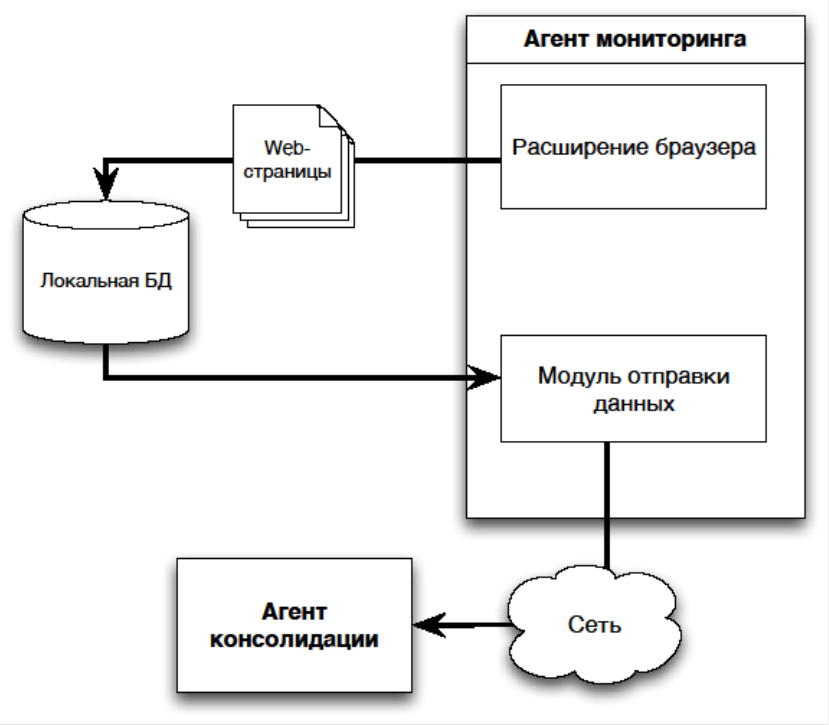
\includegraphics[width=10cm]{pic/agent1.png}
		\caption{Архитектура агента мониторинга}
		\label{fig:low_sigma}
	\end{center}
\end{figure}
Агент мониторинга состоит из нескольких компонент:
\begin{itemize}
	\item Расширение для браузера.
	\item Модуль передачи данных агенту консолидации.
\end{itemize}


Расширение для браузера, написанное с помощью BHO,  считывает html код просматриваемой пользователем веб-страницы и сохраняет ее в локальную базу данных. Сохранение в локальную базу данных осуществляется для контроля нагрузки на агент консолидации и возможности отправки данных по расписанию, а также на случай потери связи с агентом консолидации.

Модуль передачи данных агенту подключается к локальной базе данных и отправляет хранящуюся в ней информацию агенту консолидации, при получении ответа от агента консолидации отправленные данные удаляются из локальной базы данных, чтобы размер локальной базы данных не увеличивался постоянно.

Каждый из пользователей является источником собираемой информации. При этом задача требует того, чтобы пользователь не имел доступа к собираемым данным. В случае реализации агента мониторинга с помощью BHO защищенность может осуществляться с помощью установки прав доступа на папку, в которой хранятся собираемые данные.
\subsubsection {Агент консолидации}
\begin{figure}[h]
	\begin{center}
		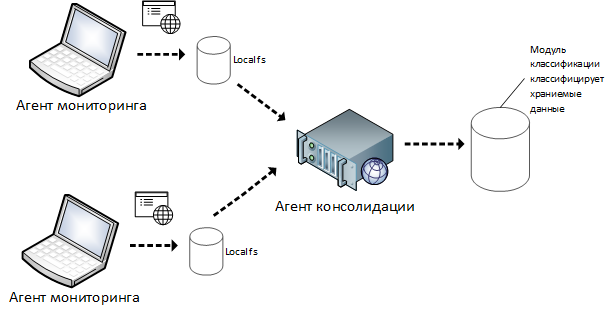
\includegraphics[width=14cm]{pic/agent2.png}
		\caption{Архитектура агента сбора}
		\label{fig:low_sigma}
	\end{center}
\end{figure}
Агент консолидации сохраняет данные, полученные от всех агентов мониторинга, в единую базу данных.Также в базу данных заносится дополнительная информация о страницах:
\begin{itemize}
	\item Логин пользователя, посещавшего веб-страницу.
	\item Имя компьютера, на котором находится пользователь.
	\item Дата посещения.
	\item ID веб-страницы.
\end{itemize}

При реализации необходимо учитывать то, что количество пользователей может быть достаточно велико, поэтому необходимо обеспечить масштабируемость агента сбора.
\subsubsection{Модуль классификации}
В ходе обзора было принято решение использовать модуль классификации, реализованный в лаборатории Технологий Программирования, основанный на подходе попарных сравнений (декомпозиция типа «каждый-против-каждого»). 

Предложенное решение включает новый алгоритм ранжирования, основанный на модифицированном для случая существенно пересекающихся классов, и новый алгоритм построения пороговой функции отсечения нерелевантных классов. 
\begin{figure}[h]
	\begin{center}
		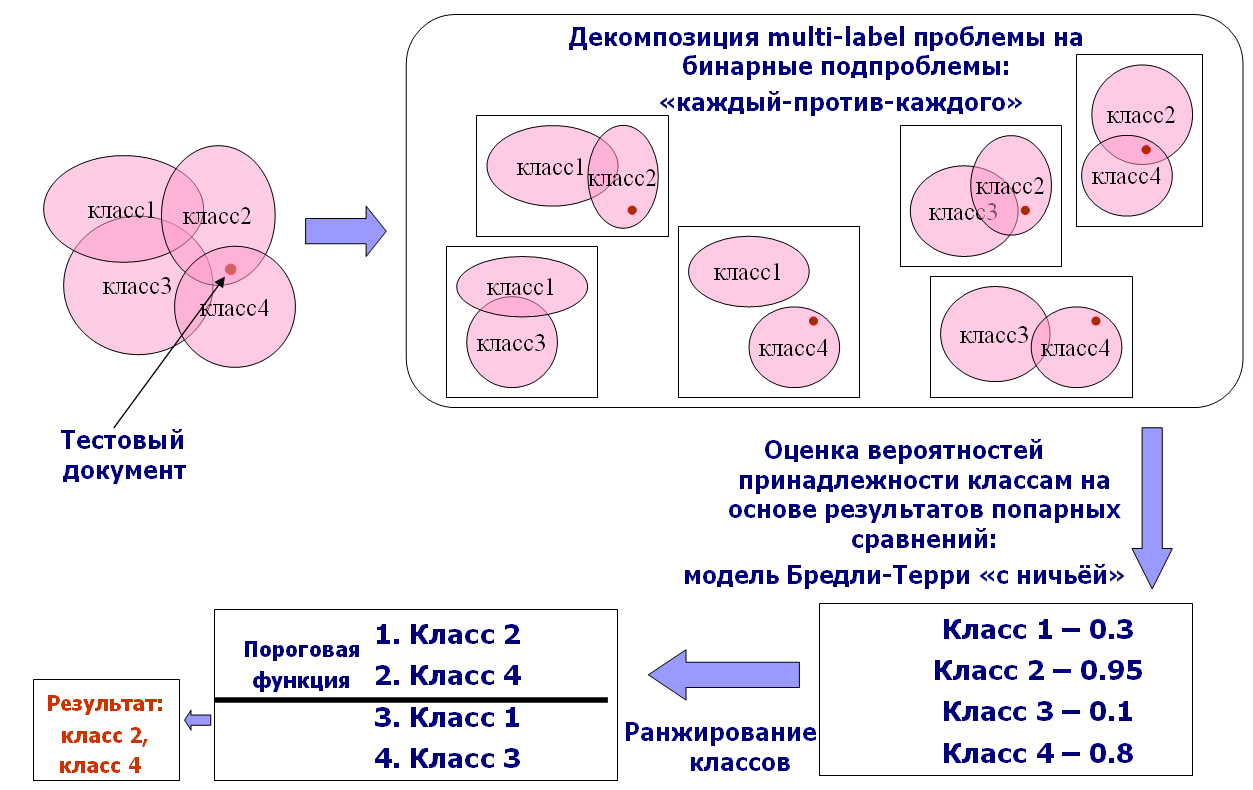
\includegraphics[width=14cm]{pic/module.png}
		\caption{Работа модуля классификации}
		\label{fig:low_sigma}
	\end{center}
\end{figure}
Он предоставляет следующие сценарии работы:
\begin{itemize}
	\item {\bf Обучение.}Построение модели классификации на основе совокупности заранее рубрицированных гипертекстовых документов.
	
	\item {\bf Классификация.}Применение построенной модели к новому классифицируемому документу.
	\item {\bf Дообучение.}Модификация модели классификации на основе дообучения на новых документах с релевантными для них тематиками.
	\item {\bf Удаление темы.}Удаление тематики классификации из модели без необходимости последующего обучения "с нуля".
\end{itemize}


\section{Описание практической части}
В данном разделе будет рассмотрена архитектура разработанного программного средства, представлен основной сценарий работы с ним, а также пояснены детали реализованных механизмов. Также будут приведены некоторые характеристики функционирования разработанного средства.
\subsection{Общая архитектура разработанного средства}
При разработке прототипа системы использовался мультиагентный подход, прототип состоит из:
\begin{itemize}
	\item Агента мониторинга.
	\item Агента консолидации.
	\item Модуля многотемной классификации.
\end{itemize}
Архитектура реализованного прототипа представлена ниже.
	\begin{figure}[h]
		\begin{center}
			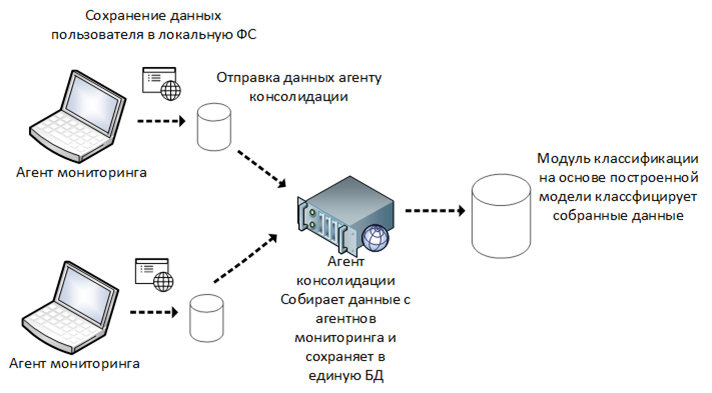
\includegraphics[width=12cm]{pic/arch.png}
			\caption{Архитектура прототипа}
			\label{fig:low_sigma}
		\end{center}
	\end{figure}
\subsubsection{Агент мониторинга}
Задача сбора просмотренных пользователем веб-страниц осуществляется с помощью расширения для браузера IE.

При открытии окна браузера расширение создает подключение к существующей базе данных, реализованной с помощью SQLite. Если базы данных нет, то создается новая, имеющая таблицу со следующими полями:
\begin{itemize}
	\item Имя пользователя
	\item Имя компьютера
	\item URL просмотренной страницы
	\item Дата
	\item HTML код страницы
\end{itemize}

Каждый раз, когда пользователь загружает новую страницу, происходит событие, по которому html код просмотренной веб-страницы сохраняется в локальную базу данных.

Расширение написано с помощью BHO (Browser Helper Object) на языке программирования C\#, объем кода - 350 строк
\subsubsection{Агент сбора}

Каждый агент, расположенный на пользовательском компьютере, подключается к базе данных, в которую были записаны данные расширением для браузера, и отправляет данные агенту сбора.

При настройке системы можно указать временной интервал, по которому будут отправляться данные. При отправке сохраняется время, когда была отправлена последняя просмотренная пользователем веб-страница.

При получении ответа от агента сбора, все записи, просмотренные до сохраненной временной метки, удаляются, так как агент сбора успешно их сохранил, если же ответ не получен, то посылаются все записи, которые хранятся в базе.

Соединение агента мониторинга и агента сбора осуществляется с помощью TCP/IP сокетов. Каждый новый агент сбора обрабатывается в агенте консолидации асинхронно в отдельном потоке, что обеспечивает высокую скорость взаимодействия.

Детали реализации модуля передачи данных агенту консолидации:
\begin{itemize}
	\item Количество строк кода - 250.
	\item Язык реализации - C\#.
	\item Доступ к локальной файловой системе без подтверждения пользователя осуществляется с помощью утилиты icacls. \cite{icacls}, которая позволяет менять Integrity Levels \cite{icacls} файлов. Так как Internet Exploler имеет право записи только в папки с Low Integrity уровнем, то для записи в нужное место необходимо создать папку и указать Integrity Level. 
\end{itemize}

Агент сбора при получении посылает ответ агенту мониторинга, закрывает соединение и записывает полученные данные в единую базу данных, при этом к каждой записи добавляется ID.

Детали реализации агента консолидации:
\begin{itemize}
	\item Агент сбора был написан на примере асинхронного сокет сервера \cite{msdn}
	\item Язык написания - С\#
	\item Количество строк кода - 600
\end{itemize}
\subsubsection{Модуль многотемной классификации}
С учетом требований, сформулированных в постановке задачи, для многотемной классификации был выбран модуль, разработанный в лаборатории Технологий Программирования.
Модуль многотемной классификации состоит из:
\begin{itemize}
	\item компонент лексического анализа (парсер) – осуществляет разбор, выделение признаков и преобразование гипертекстовых документов во внутреннее представление;
	\item компонент вычисления меры сходства – определяет значения близости между документами (значения функции ядра) на основе выданного парсером представления и осуществляет кэширование этих значений; 
	\item классификатор – строит дообучаемую модель классификации и на её основе осуществляет классификацию многотемных гипертекстовых документов.
\end{itemize}
 \begin{figure}[h]
 	\begin{center}
 		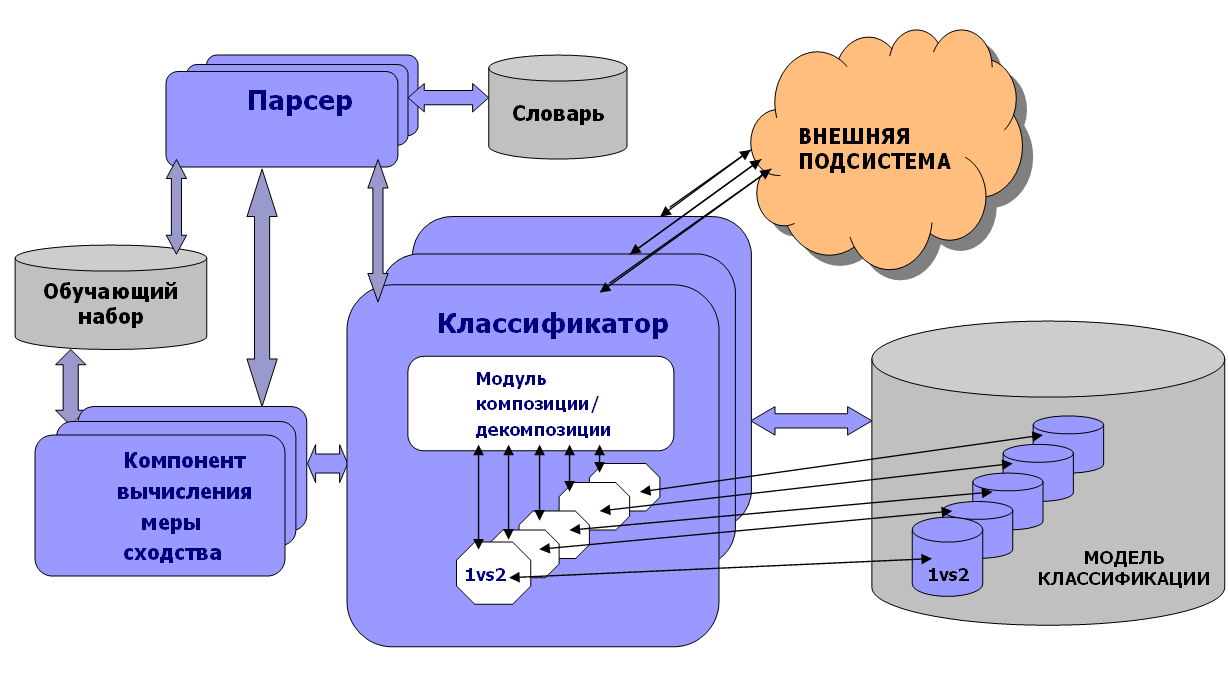
\includegraphics[width=14cm]{pic/module2.png}
 		\caption{Архитектура модуля классификации}
 		\label{fig:low_sigma}
 	\end{center}
 \end{figure}
 
Для интеграции системы сбора с модулем многотемной классификации был написан модуль, который позволяет:
\begin{itemize}
\item Производить парсинг html кода страницы.
\item Обучать классификатор, подавая ему на вход тренировочный набор, содержащий веб-страницу и тематику, к которой данный документ принадлежит.
\item Выгружать веб-страницы из заданной базы данных и подавать их на вход классификатору. На выходе создается .csv файл с весами тематик для каждого документа.
\end{itemize}

Модуль написан на языке программирования Python, объем - 200 строк
\subsection{Экспериментальные исследования}
В ходе обзора существующих решений было выдвинуто требование масштабируемости агента консолидации.

	
Так как разработка велась на языке программирования C\# в среде разработки Visual Studio, то для проведения нагрузочного тестирования было решено воспользоваться встроенными средствами Visual Studio \cite{test}.

Ход тестирования:
\begin{itemize}
	\item Для нагрузочного тестирования были созданы Unit тесты \cite{unitTest}, содержащие код компоненты агента мониторинга, который взаимодействует с агентом консолидации
	\item Visual Studio позволяет выбирать такие параметры сценария тестирования как: начальное количество клиентов, максимально количество клиентов, и скорость увеличения
	количества клиентов.
	\item Далее, задавая параметры сценариев, было проведено исследование зависимости нагрузки ЦП и оперативной памяти от количества подключенных клиентов.
	 \begin{figure}[h]
	 	\begin{center}
	 		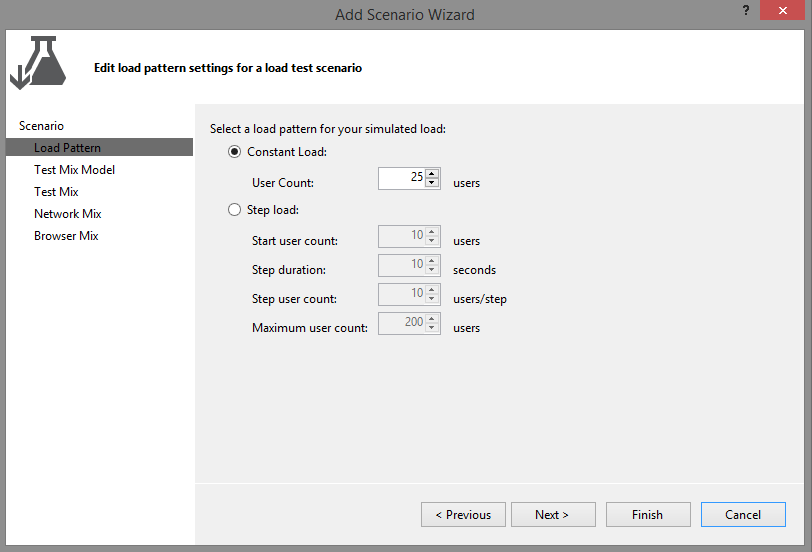
\includegraphics[width=14cm]{pic/test.png}
	 		\caption{Параметры сценария тестирования}
	 		\label{fig:low_sigma}
	 	\end{center}
	 \end{figure}
\end{itemize}
\subsubsection {Исследование зависимости нагрузки ЦП от количества подключенных клиентов}

Сценарий тестирования:
\begin{itemize}
	\item Начальное количество клиентов - 1. Каждый подключенный клиент с заданной частотой посылает агенту консолидации просмотренные пользователем веб-страниц.
	\item С установленной скоростью увеличивается количество подключенных агентов мониторинга.
	\item С помощью средств Visual Studio отрисовывается график, отражающий зависимость нагрузки ЦП от количества подключенных клиентов.
\end{itemize}

Результаты тестирования проиллюстрированы ниже
 \begin{figure}[h]
 	\begin{center}
 		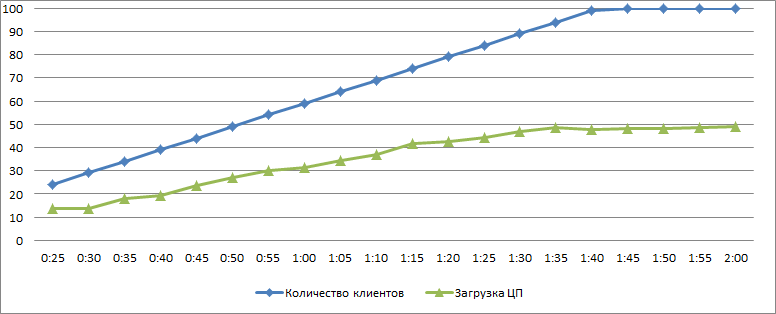
\includegraphics[width=12cm]{pic/test1.png}
 		\caption{Зависимость нагрузки ЦП от количетва клиентов}
 		\label{fig:low_sigma}
 	\end{center}
 \end{figure}
 
\subsubsection{Исследование использования оперативной памяти от количества клиентов}

Сценарий тестирования аналогичен сценарию из предыдущего пункта.
Результаты тестирования приведены ниже:
\begin{figure}[h]
	\begin{center}
		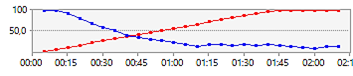
\includegraphics[width=12cm]{pic/test2.png}
		\caption{Зависимость использования оперативной памяти от количества клиентов}
		\label{fig:low_sigma}
	\end{center}
\end{figure}
\subsection{Результаты тестирования}

Зависимость нагрузки центрального процессора от количества подключенных клиентов линейна, что говорит о масштабируемости разработанного средства.

Увеличение использования оперативной памяти при увеличении количества подключенных клиентов  линейно, что также говорит о масштабируемости разработанного средства.
\section {Заключение}
В настоящей выпускной квалификационной работе были проведены исследования методов многотемной классификации веб-страниц.В ходе работ обозревали современные индустриальные системы, которые решают ряд задач, требующих сбор и классификации веб-страниц, с которыми работали пользователи.Были рассмотрены различные подходы к классификации текстовых данных: методов шаблонов, метод цифровых, методы на основе машинного обучения. Было принято решение, что требованиям поставленной задачи удовлетворяет только методы, основанные на машинном обучении. 

Был проведен анализ основных подходов к решению задачи многотемной классификации: "оптимизационный" подход, подход на основе декомпозиции в набор независимых бинарных проблем, подход на основе ранжирования, выявлены недостатки, не позволяющие применять их для решения поставленной задачи. Также был рассмотрен и выбран метод многотемной классификации на основе подхода попарных сравнений, учитывающий недостатки традиционных подходов.



Была осуществлена программная реализация прототипа системы сбора и многотемной классификации веб-страниц, состоящей из:
\begin{itemize}
	\item Агента мониторинга.
	\item Агента консолидации.
	\item Модуля многотемной классификации.
\end{itemize}

С помощью средств модульного и нагрузочного тестирования, предоставленного средой Miscrosoft Visual Studio были реализованы сценарии нагрузочного тестирования и измерены следующие параметры функционирования разработанного прототипа системы:
\begin{itemize}
	\item Зависимость нагрузки центрального процессора от количества подключенных клиентов.
	\item Зависимость количества свободной оперативной памяти от количества подключенных клиентов.
\end{itemize}

Результаты тестирования показали линейный рост нагрузки центрального процесса при увеличении количества подключенных клиентов, что говорит о масштабируемости разработанного прототипа.

Также результаты тестирования показали линейное убывание свободной оперативной памяти при увеличении количества клиентов, что говорит о масштабируемости.

Реализация сбора данных с помощью BHO позволила сохранять данные о просмотренных пользователем веб-страницах в локальную файловую систему в директорию с ограниченным правом доступа, что обеспечивает защищенность (обычный пользователь не имеет доступа к собранным данным) разработанного прототипа.
\begin{thebibliography}{50}
	\bibitem{InfoWatch}
	\textit {Аналитический Центр InfoWatch, Безопасность информации в корпоративных информационных системах. Внутренние угрозы}
	{(http://www.infowatch.ru/analytics/reports/4609)}
	\bibitem{ContentClassification}
	\textit {Component overview (Content Classification 8.8.0)}
	\bibitem{eDiscovery}
	\textit{Electronic discovery.}
	{(wikipedia.org/wiki/Electronic\_discovery)}
	\bibitem{Symantec}
	\textit {Предиктивное обучение}
	{(http://www.symantec.com/ru/ru/predictive-coding/)}
	\bibitem{bkf}
	\textit {Infowatch БКФ }
	{(http://www.infowatch.ru/technologies)}
	\bibitem {searcher}
	\textit{text}{122.	Component overview (IBM Watson Content Analytics 3.5.0)}
	{(http://www-01.ibm.com/support/knowledgecenter/SS5RWK\_3.5.0/com.ibm.discovery.es.nav.doc/iiysaovcomp.htm?lang=en)}
	\bibitem{analitic}
	\textit{Официальная документация IBM в Интернет}
	{(http://www-01.ibm.com/support/knowledgecenter/SS5RWK\_3.5.0/com.ibm.discovery.es.nav.doc/iiysaovcomp.htm?lang=en)}
	\bibitem{idx1}
	\textit{Content Analytics. Официальный сайт OpenText в Интернет}
	{(http://www.opentext.com/what-we-do/products/discovery/content-analytics)}
	\bibitem{idx2}
	\textit{EMC Kazeon File Intelligence}
	{(http://www.emc.com/content-management/emc-kazeon-file-intelligence.htm)}
	\bibitem{wikiAdaBoost}
	\textit{Работа AdaBoost алгоритма}
	{(https://ru.wikipedia.org/wiki/AdaBoost)}
	\bibitem{idx3}
	\textit{Using the Taxonomy Proposer to discover new categories}
	{(http://www-01.ibm.com/support/knowledgecenter/}
	\bibitem{MachLearn}
	\textit {Symantec Machine Learning}
	{(http://eval.symantec.com/mktginfo/enterprise/)}
	\bibitem{SVM}
	\textit{Boutell M. R., Luo J., Shen X., Brown C.M. Learning multi-label scene classification }
	{Pattern Recognition. 2004. №37. pp. 1757-1771.}
	\bibitem{msdn}
	\textit{Асинхронный сокет сервер}
	{(https://msdn.microsoft.com/ru-ru/library/fx6588te(v=vs.110).aspx)}
	\bibitem{DOM}
	\textit{Document Object Model}
	{https://ru.wikipedia.org/wiki/Document\_Object\_Model}
	\bibitem{icacls}
	\textit{Утилита icacls}
	{(https://msdn.microsoft.com/en-us/library/bb625965.aspx)}
	\bibitem{unitTest}
	\textit{Create and run unit tests.}
	{(https://www.visualstudio.com/en-us/get-started/code/create-and-run-unit-tests-vs)}
	\bibitem{test}
	\textit{Walkthrough: Creating and Running a Load Test Containing Unit Tests}
	{(https://msdn.microsoft.com/en-us/library/vstudio/ff355993(v=vs.110).aspx)}
	\bibitem{tan}
	\textit{Таненбаум Э., Ван Стеен М.}
	{Распределенные системы. Принципы и парадигмы}
	\bibitem{AdaBoost}
	\textit{Schapire R. E., Singer Y. BoosTexter}
	{A boosting-based system for text categorization}
	\bibitem{ADT}
	{Comite F. D., Gilleron R., Tommasi M. Learning multi-label alternating decision tree from texts and data}
	{Machine Learning and Data Mining in Pattern Recognition, MLDM 2003 Proceedings, Lecture Notes in Computer Science 2734. Berlin, 2003. pp. 35–49s}
	\bibitem{kNN}
	\textit{Zhang M.-L., Zhou Z.-H. A k-nearest neighbor based algorithm for multi-label classification }
	{Proceedings of the 1st IEEE International Conference on Granular Computing (GrC'05). Beijing, China, 2005. pp. 718-721}
	\bibitem{MMP1}
	\textit{C. Crammer, Y. Singer. A family of additive online algorithms for category ranking}
	{Machine Learning Research. №3. 2003. pp. 1025–1058}
	\bibitem{MMP2}
	\textit{Crammer C., Singer Y. A new family of online algorithms for category ranking }
	{Proceedings of the 25th annual international ACM SIGIR conference on Research and development in information retrieval. Tampere, Finland, 2002. pp. 151 – 158}
	\bibitem{kNN3}
	\textit{Minh Duc Cao, Xiaoying Gao. Combining Content and Citation for Scientific Document Classification}
	{AI2005, LNAI 3809, 2005. pp. 143-152}
	\bibitem{bredli}
	{P.V. Rao and L.L. Kupper. Ties in paired-comparison experiments}
	{A generalization of the Bradley–Terry model, Amer. Statist. Assoc, 62, 1967. pp. 194–204.}
	\bibitem{dis}
	\textit{Глазкова В.В.}
	{Исследование и разработка методов построения программных средств классификации многотемных гипертекстовых документов}
	\bibitem{mlKNN}
	\textit{Zhang M.-L., Zhou Z.-H. A k-nearest neighbor based algorithm for multi-label classification }
	{Proceedings of the 1st IEEE International Conference on Granular Computing (GrC'05). Beijing, China, 2005. pp. 718-721}
	\bibitem{rank1}
	\textit{C. Crammer, Y. Singer. A family of additive online algorithms for category ranking}
	{Machine Learning Research. №3. 2003. pp. 1025–1058}
	\bibitem{rank2}
	\textit{Minh Duc Cao, Xiaoying Gao. Combining Content and Citation for Scientific Document Classification}
	{AI2005, LNAI 3809, 2005. pp. 143-152.}
\end{thebibliography}
\end{document}